\documentclass{article}

\usepackage{amsmath, amssymb}
\usepackage{tikz}

\newcommand{\R}{\mathbb R}
\newcommand{\Z}{\mathbb Z}

\DeclareMathOperator{\im}{im}

\title{Simplicial Homology and Cohomology\\ A Geometrical Introduction}
\author{Sebastián Sánchez}

\begin{document}

\maketitle

\section{Introduction}

Rigorous definition are based on~\cite{munkres}.

\section{Simplicial Complexes}

A simplicial complex is a generalization of a triangulation. The role of triangles is
played by the simplices. A \(d\)-simplex is collection of \(d+1\) affinely independent points
in \(\R^{d}\), affinely indepedent means that the relative vectors are linearly independent:
\begin{displaymath}
  a_0, \dots, a_d \quad\textrm{affinely independent}
  \iff
  a_1-a_0, \dots, a_d-a_0 \quad\textrm{linearly independent}.
\end{displaymath}
Naturally, we can associate a geometric realization of a simplex by taking is convex hull.
A simplicial complex \(K\) is a collection of simplices closed under the relation of subsets and 
closed under the operation of intersection. Explicitely,
\begin{enumerate}
  \item for any \(P\in K\), \(Q\in K\) for any \(Q\subset P\),
  \item for any \(P, S\in K\), \(P\cap S \in K\).
\end{enumerate}

\section{Simplicial Homology}

We start with the usual introduction to simplicial homology and then move into
the geometry.

\subsection{Notation and Definitions}

Let \(K\) be a simplicial complex and give it an orientation. That is, every
simplex now is not just a set, but an ordered list. We declare two orientations
of a simplex to be the same if they differ by an even permutation. Define the
oriented indicator function of an (oriented) simplex \(P\) as follows:
\begin{displaymath}
  c_P(Q) =
  \left\{
  \begin{aligned}
    1 &\quad \textrm{if } Q=P\\
    -1 &\quad \textrm{if } Q=P\text{ as sets but differ in orientation}\\
    0 &\quad \textrm{if} Q\ne P
  \end{aligned}.
  \right.
\end{displaymath}
Let \(K^{(d)}\) be the simplices of dimension \(d\) of \(K\). A \(d\)-chain is
a linear function from \(K^{(d)}\) to \(R\), where \(R\) is a conmutative ring with unity
(I prefer to just set it to \(\R\)).
The set of all \(d\)-chains is denoted as \(C_d(K)\) and have a group structure
when coupled with point-wise addition. Then, every element can be written as:
\begin{displaymath}
  c\in C_d(K) \iff c = \sum_{P\in K^{(d)}} \alpha_P c_P
  \quad \alpha_P\in R.
\end{displaymath}
The about equations says that the group is free and that the oriented indicators are a basis.
Define the linear map \(\partial_d\colon C_d \to C_{d-1}\) acting as
\begin{displaymath}
  \partial_d [p_0, \ldots, p_d] = \sum_{i=0}^{d} (-1)^{i} [p_0, \ldots, \hat p_i, \ldots, p_d]
\end{displaymath}
where \(\hat p_i\) means that we remove that element from the ordered list and we have identified
the simplices with their indicators.
This map is called the boundary map and satisfies \(\partial_{d} \circ
\partial_{d-1} = 0\). Finally, define the \(d\)-homology group as
\begin{displaymath}
  H_d(K) = \frac{\ker \partial_{d}}{\im \partial_{d+1}}.
\end{displaymath}

\subsection{Geometry}

A \(d\)-chain is a selection of simplices (by definition) and can be thought as a 
subcomplex or even a \(d\)-dimensional walk. Let's start simple. Consider the simplicial
complex shown below.

\begin{center}
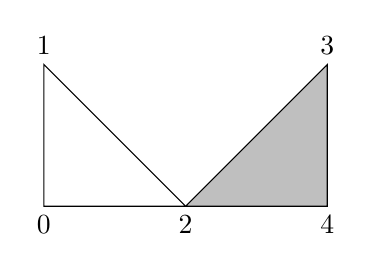
\begin{tikzpicture}[scale=1.8]
  \draw[fill=gray!50!white] (1, 0) -- (2, 1) node[above] {3} -- (2, 0) node[below] {4} -- cycle; 
  \draw (0,0) node[below] {0} -- (0,1) node[above] {1} -- (1,0) node[below] {2} -- cycle;
\end{tikzpicture}
\end{center}

There is 1 simplex of dimension 2, 6 simplices of dimension 1 and 5 simplices of dimension 0,
corresponding to the filled triangle, the edges and the points, respectively. We give the 
increasing index orientation. Consider the subcomplex given by \([0,1], [1,2], [2,0]\).
The corresponding chain is
\begin{displaymath}
  c = [0,1] + [1,2] - [0, 2].
\end{displaymath}
Then, evaluation of \(c\) ask for membership. Let's see what the boundary operator does to this
subcomplex:
\begin{displaymath}
  \partial c = ([0] - [1]) + ([1] - [2]) - ([0] - [2]) = 0
\end{displaymath}
That is, the boundary of \(c\) has no members. Let's compute a different example. Consider
the chain:
\begin{displaymath}
  c' = [0, 2] + [2, 4]
\end{displaymath}
Then, \(\partial c' = [0] + [4]\) and the boundary of \(c'\) has as members 0 and 4.
Therefore, as the name suggest, the boundary map computes the boundary of the subgraph
and having no boundary means we are in a cycle.


\section{Simplicial Cohomology}

\begin{thebibliography}{9}
\bibitem{munkres}
  Elements of Algebraic Topology (1989), James Munkres.
\end{thebibliography}

\end{document}
